\begin{name}
	{\tenchude}
	{\tendethi}
	{\tentruong}
	{\thoigian}
\end{name}
\setcounter{ex}{0}\setcounter{bt}{0}
\TN
\Opensolutionfile{ans}[ans/ansDe1-TN1]
\begin{ex}%[2-D1B1-SO-2-2425]%[VN-MT-018]%[2D1N1-1]
	Cho hàm số $y=x^3+3x+2$. Mệnh đề nào dưới đây là đúng?
	\choice
	{\True Hàm số đồng biến trên khoảng $(-\infty ;+\infty )$}
	{Hàm số nghịch biến trên khoảng $(-\infty ;+\infty )$}
	{Hàm số nghịch biến trên khoảng $(-\infty ;0)$ và đồng biến trên khoảng $(0;+\infty )$}
	{Hàm số đồng biến trên khoảng $(-\infty ;0)$ và nghịch biến trên khoảng $(0;+\infty )$}
	\loigiai{
		Tập xác định $\mathscr{D}=\mathbb{R}$.\\
		Ta có $y'=3x^2+3>0$, $\forall x\in \mathbb{R}$ suy ra hàm số đồng biến trên khoảng $(-\infty ;+\infty )$.}
\end{ex}

\begin{ex}%[2D1N1-2]
	Cho hàm số $y=f(x)$ có bảng biến thiên như sau.
	\begin{center}
		\begin{tikzpicture}[>=stealth, scale=1,line join=round, line cap=round, font=\footnotesize]
			\tkzTabInit[lgt=1.2,espcl=2.3]
			{$x$/0.8,$y'$/0.8,$y$/3}
			{$-\infty$,$-2$,$3$,$+\infty$}
			\tkzTabLine{,-,0,+,0,-,}
			\path
			(N12)node[shift={(0,-0.2)}](A){$+\infty$}
			(N23)node[shift={(0,0.8)}](B){$1$}
			(N32)node[shift={(0,-0.8)}](C){$4$}
			(N43)node[shift={(0,0.2)}](D){$-\infty$};
			\foreach\X/\Y in{A/B,B/C,C/D}\draw[->](\X)--(\Y);
		\end{tikzpicture}
	\end{center}
	Hàm số đã cho đồng biến trên khoảng nào dưới đây?
	\choice
	{$(3;+\infty)$}
	{$(-\infty;-2)$}
	{$(-2;+\infty)$}
	{\True $(-2;3)$}
	\loigiai{
		Hàm số đã cho đồng biến trên khoảng	$(-2;3)$.
	}
\end{ex}

\begin{ex}%[CD12-KNTT, Mức độ 3]%[2D1V1-5]
	Nhân dịp Ngày Quốc tế phụ nữ $8$ - $3$, câu lạc bộ mĩ thuật của An muốn tổ chức kinh doanh thiệp chúc mừng ngày $8$ - $3$ để gây quỹ sinh hoạt cho câu lạc bộ. Mỗi tấm thiệp mua về với giá $8$ nghìn đồng. Các bạn trong câu lạc bộ sẽ sáng tác thêm nội dung của thiệp (vẽ thêm hình ảnh người, hoa cỏ, lời chúc \ldots) và sau đó bán lại. Với mức giá bán $20$ nghìn đồng cho $1$ tấm thiệp, câu lạc bộ có thể bán được $500$ chiếc. Cứ với mỗi $1$ nghìn đồng giảm giá, số lượng hàng bán ra tăng thêm $50$ chiếc. Phát biểu nào sau đây là \textbf{đúng}?
	\choice
	{\True Khi giá giảm từ $1$ nghìn đồng đến $20$ nghìn đồng thì lợi nhuận của câu lạc bộ sẽ giảm}
	{Khi giá giảm từ $5$ nghìn đồng đến $20$ nghìn đồng thì lợi nhuận của câu lạc bộ không đổi}
	{Khi giá giảm từ $1$ nghìn đồng đến $20$ nghìn đồng thì lợi nhuận của câu lạc bộ sẽ tăng}
	{Khi giá giảm từ $5$ nghìn đồng đến $20$ nghìn đồng thì lợi nhuận của câu lạc bộ sẽ tăng}
	\loigiai{
		Gọi $x$ (nghìn đồng) là số tiền giảm giá cho mỗi tấm thiệp, $0\le x\le 20$.\\
		Số lượng tấm thiệp bán ra là $500+50x$ (chiếc).\\
		Hàm chi phí cho $500+50x$ tấm thiệp là $(500+50x)\cdot 8$ (nghìn đồng).\\
		Hàm doanh thu cho $500+50x$ tấm thiệp là $(500+50x)(20-x)$ (nghìn đồng).\\
		Khi đó lợi nhuận thu được là
		\allowdisplaybreaks
		\begin{eqnarray*}
			P(x)&=&(20-x)(500+50x)-8(500+50x)\\
			&=& (12-x)(500+50x)\\
			&=& 6\,000+100x-50x^2\text{ (nghìn đồng).}
		\end{eqnarray*}
		Để tối đa hóa lợi nhuận, thì ta phải tìm giá trị lớn nhất của hàm $P(x)$ với $0\le x\le 20$.\\
		Ta có $P'(x)=100-100x=0$ khi $x=1$. \\
		Khi đó $P(1)=6\,050$ (nghìn đồng) là giá trị lớn nhất của hàm lợi nhuận, đạt được khi $x=1$. \\
		Tức là khi giá giảm từ $1$ nghìn đồng đến $20$ nghìn đồng thì lợi nhuận của câu lạc bộ sẽ giảm.
	}
\end{ex}

\begin{ex}%[Mức độ 1]%[2D1N2-1]
	Hàm số $y=x^2$ có cực tiểu tại
	\choice
	{\True $x=0$}
	{$x=1$}
	{$x=2$}
	{$x=3$}
	\loigiai
	{
		Ta có $y'=2x$.\\
		$y'=0\Leftrightarrow x=0$\\
		$y'$ đổi dấu từ âm sang dương khi đi qua $x=0$ nên hàm số đạt cực tiểu tại $x=0$
	}
\end{ex}

\begin{ex}%[EX-Ôn Tập TN 2025, PT Sinh]%[2D1N2-2]
	\immini{Cho hàm số $y = f(x)$ có đồ thị như hình vẽ. Điểm cực tiểu của đồ thị hàm số đã cho là
		\choice[2]
		{$(-1; 0)$}
		{$(1; 0)$}
		{$(2; 0)$}
		{\True $(1; -4)$}
	}{
		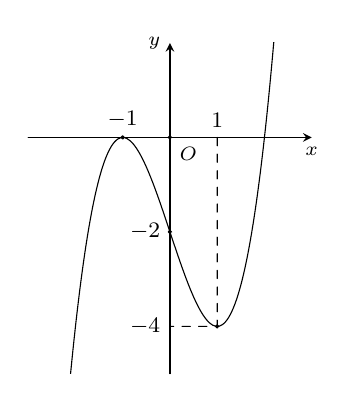
\begin{tikzpicture}[scale=0.6, font=\footnotesize, line join=round, line cap=round, >=stealth,x=1cm,y=1cm]
			\def\a{1} % Hệ số a phải khác 0
			\def\b{0}
			\def\c{-3}
			\def\d{-2}
			%\draw[color=gray,dash pattern=on 1pt off 1pt,xstep=1.0cm,ystep=1.0cm] (-5.2,-5.2) grid (5.2,5.2);
			\draw[->] (-3,0) -- (3,0)node[below]{\scriptsize $x$};
			\draw[->] (0,-5) -- (0,2) node[left] {\scriptsize $y$};
			\draw (0,0)node[below right]{\scriptsize $O$};
			\clip (-3,-5)rectangle(3,2);
			\draw[samples=150,smooth,domain=-5:5] plot(\x,{\a*(\x)^3+(\b)*(\x)^2+(\c)*\x+(\d)});
			\fill[black] (0,0) circle(1.0pt);
			\draw [dashed] (1,0)--(1,-4)--(0,-4) (0,-4) node[left]{$-4$} (0,-2) node[left]{$-2$} circle (1pt) (1,0) node[above]{$1$}  (-1,0) node[above]{$-1$} circle (1pt) (1,-4)circle(1pt) (0,0)circle(1pt);
		\end{tikzpicture}
	}
	\loigiai{Điểm cực tiểu của đồ thị hàm số đã cho là $(1; -4)$.
	}
\end{ex}

\begin{ex}%[2-D1B5-SO-14-2425]%[VN-MT-7, Đỗ Minh Phúc]%[2D1H2-1]
	Hàm số $f(x)=x^3-3x^2-9x+1$ đạt cực đại tại điểm
	\choice
	{\True $x=-1$}
	{$x=1$}
	{$x=3$}
	{$x=-3$}
	\loigiai{
		Ta có $f'(x)=3x^2-6x-9$.\\
		Cho $f'(x)=0\Leftrightarrow 3x^2-6x-9=0\Leftrightarrow\hoac{&x=-1\\&x=3.}$\\
		Ta có bảng biến thiên
		\begin{center}
			
\begin{tikzpicture}
				\tkzTabInit[nocadre,lgt=1.2,espcl=2.5,deltacl=0.6]
				{$x$/0.6,$y'$/0.6,$y$/2}
				{$-\infty$,$-1$,$3$,$+\infty$}
				\tkzTabLine{,+,0,-,0,+,}
				\tkzTabVar{-/$-\infty$,+/$6$,-/$-26$,+/$+\infty$}
			\end{tikzpicture}
		\end{center}
		Dựa vào bảng biến thiên, ta thấy hàm số đạt cực đại tại $x=-1$.
	}
\end{ex}

\begin{ex}%[2D1H3-1]
	Tìm giá trị lớn nhất của hàm số $f(x)=\sin x+\cos 2x$ trên $\left[0;\pi \right]$ là
	\choice
	{\True $\dfrac{9}{8}$}
	{$\dfrac{5}{4}$}
	{$2$}
	{$1$}
	\loigiai{
		$f(x)=\sin x+\cos 2x=\sin x+1-2\sin^2x$. \\
		Đặt $\sin x=t\left(0\leqslant t\leqslant 1\right)$. \\
		$g(t)=-2t^2+t+1$, $g'(t)=-4t+1$. \\
		$g'(t)=0 \Leftrightarrow t=\dfrac{1}{4}$. \\
		$g(0)=1$, $f(1)=0$, $g\left(\dfrac{1}{4}\right)=\dfrac{9}{8}$. \\
		Vậy $\displaystyle\max _{[0;1]}f(x)=\dfrac{9}{8}$.}
\end{ex}

\begin{ex}%[2D1N4-1]
	Trong không gian $Oxyz$ (đơn vị của các trục tọa độ là kilomet), một trạm thu phát sóng điện thoại di động có đầu thu phát được đặt tại điểm $I(6;-2;4)$. Cho biết bán kính phủ sóng của trạm là $6$km. Viết phương trình mặt cầu $(S)$ biểu diễn ranh giới của vùng phủ sóng.
	\choice
	{$(x-6)^2+(y+2)^2+(z-4)^2=6$}
	{\True $(x-6)^2+(y+2)^2+(z-4)^2=36$}
	{$(x+6)^2+(y-2)^2+(z+4)^2=6$}
	{$(x+6)^2+(y-2)^2+(z+4)^2=36$}
	\loigiai{
		Mặt cầu (S) có tâm $I(6;-2;4)$ và bán kính $R=6$ nên có phương trình:\\
		$(x-6)^2+(y+2)^2+(z-4)^2=36$.
	}
\end{ex}

\begin{ex}%[2-D1B5-SO-16-2425]%[VN-MT-7, Dương Phước Sang]%[2D1H4-1]
	Đường thẳng nào sau đây là tiệm cận xiên của đồ thị hàm số $y=\dfrac{2x^2-3x+1}{x+2}$?
	\choice
	{$y=2x$}
	{$y=2$}
	{\True $y=2x-7$}
	{$x=-2$}
	\loigiai{
		Ta có $y=f(x)=\dfrac{2x^2-3x+1}{x+2}=2x-7+\dfrac{15}{x+2}$.\\
		$\lim\limits_{x \to \pm\infty} [f(x)-(2x-7)]=\lim\limits_{x \to \pm\infty} \dfrac{15}{x+2}=0$.\\
		Vậy đồ thị hàm số có tiệm cận xiên là $y=2x-7$.
	}
\end{ex}

\begin{ex}%[2D1V4-1]
	Đồ thị hàm số $y=\dfrac{\sqrt{4x^2+2x-1}+x}{x+1}$ có bao nhiêu đường tiệm cận?
	\choice
	{$1$}
	{$0$}
	{\True $2$}
	{$3$}
	\loigiai{
		Hàm số $y=\dfrac{\sqrt{4x^2+2x-1}+x}{x+1}$ xác định $\Leftrightarrow \heva{&4x^2+2x-1\ge 0 \\&x+1\ne 0}\Leftrightarrow \heva{&\hoac{&x\le \dfrac{-1-\sqrt{5}}{4} \\&x\ge \dfrac{-1+\sqrt{5}}{4}} \\&x\ne -1.}$\\
		Tập xác định của hàm số là $\mathscr{D}=\left(-\infty;-1\right)\cup \left(-1;\dfrac{-1-\sqrt{5}}{4}\right]\cup \left[\dfrac{-1+\sqrt{5}}{4};+\infty\right)$.\\
		$\begin{aligned}[t]
				\underset{x\to -\infty}{\mathop{\lim}}y & =\underset{x\to -\infty}{\mathop{\lim}}\dfrac{\sqrt{4x^2+2x-1}+x}{x+1}=\underset{x\to -\infty}{\mathop{\lim}}\dfrac{\left| x\right|\sqrt{4+\dfrac{2}{x}-\dfrac{1}{x^2}}+x}{x+1}                        \\
				                                        & =\underset{x\to -\infty}{\mathop{\lim}}\dfrac{-x\sqrt{4+\dfrac{2}{x}-\dfrac{1}{x^2}}+x}{x+1}=\underset{x\to -\infty}{\mathop{\lim}}\dfrac{-\sqrt{4+\dfrac{2}{x}-\dfrac{1}{x^2}}+1}{1+\dfrac{1}{x}}=-1.\end{aligned}$\\
		Suy ra $y=-1$ là đường tiệm cận ngang của đồ thị hàm số khi $x\to -\infty $.\\
		$\begin{aligned}[t]
				\underset{x\to +\infty}{\mathop{\lim}}y & =\underset{x\to +\infty}{\mathop{\lim}}\dfrac{\sqrt{4x^2+2x-1}+x}{x+1}=\underset{x\to +\infty}{\mathop{\lim}}\dfrac{\left| x\right|\sqrt{4+\dfrac{2}{x}-\dfrac{1}{x^2}}+x}{x+1}                     \\
				                                        & =\underset{x\to +\infty}{\mathop{\lim}}\dfrac{x\sqrt{4+\dfrac{2}{x}-\dfrac{1}{x^2}}+x}{x+1}=\underset{x\to -\infty}{\mathop{\lim}}\dfrac{\sqrt{4+\dfrac{2}{x}-\dfrac{1}{x^2}}+1}{1+\dfrac{1}{x}}=3.\end{aligned}$\\
		Suy ra $y=3$ là đường tiệm cận ngang của đồ thị hàm số khi $x\to +\infty $.\\
		$\begin{aligned}[t]
				\underset{x\to -1}{\mathop{\lim}}y & =\underset{x\to -1}{\mathop{\lim}}\dfrac{\sqrt{4x^2+2x-1}+x}{x+1}=\underset{x\to -1}{\mathop{\lim}}\dfrac{4x^2+2x-1-x^2}{\left(x+1\right)\left(\sqrt{4x^2+2x-1}-x\right)} \\
				                                   & =\underset{x\to -1}{\mathop{\lim}}\dfrac{\left(x+1\right)\left(3x-1\right)}{\left(x+1\right)\left(\sqrt{4x^2+2x-1}-x\right)}=-2\end{aligned}$.\\
		Suy ra đồ thị hàm số không có tiệm cận đứng.\\
		Vậy đồ thị hàm số $y=\dfrac{\sqrt{4x^2+2x-1}+x}{x+1}$ có $2$ đường tiệm cận.}
\end{ex}

\begin{ex}%[2-D1B4-SO-12-2425]%[VN-MT-7, VM22]%[2D1N5-1]
	\immini[thm]{Cho hàm số $y=ax^3+bx^2+cx+d$ có đồ thị như hình bên.
		Khẳng định nào sau đây đúng?
		\choice[2]
		{\True $d<0$}
		{$d>0$}
		{$d=0$}
		{$d\leq 0$}
	}{
		\begin{tikzpicture}[>=stealth,scale=1.0]
			\draw[->] (-2,0)--(3,0)node[below]{$x$};
			\draw[->] (0,-1.5)--(0,2)node[left]{$y$};
			\draw[samples=100,domain=2.21:-1.33] plot (\x,{-0.83*(\x)^3+1.13*(\x)^2+1.42*(\x)-0.72});
			\draw(0,0)node[below left]{$O$};
			\fill (0,0) circle (1.0pt);
		\end{tikzpicture}
	}

	\loigiai{
		Đồ thị cắt trục tung tại điểm có tung độ âm nên $d<0$.\\
	}
\end{ex}

\begin{ex}%[Dự Án Giảng 12 4 in 1, Lê Văn Toàn]%[2D1N5-7]
	Cho hàm số $y=\dfrac{2x-1}{x-1}$ có đồ thị $(C)$. Có bao nhiêu cặp điểm $M$, $N$ nằm trên $(C)$ đối xứng nhau qua điểm $I(1;2)$?
	\choice
	{$0$}
	{$1$}
	{$2$}
	{\True Vô số}
	\loigiai{
		Ta có $I(1;2)$ là giao điểm của hai đường tiệm cận của $(C)$.
	}
\end{ex}

\begin{ex}%[2D1H5-1]%[KNTT - Lớp 12 - Ôn tập cuối học kì 1 - Đề 4]%[Phúc Hậu]
	\immini[thm]{Đồ thị như hình vẽ là đồ thị của hàm số nào dưới đây?
		\choice
		{\True $y=-x^3+3x^2-4$}
		{$y=-x^3-3x^2-4$}
		{$y=x^3-3x^2+4$}
		{$y=x^3-3x^2-4$}}{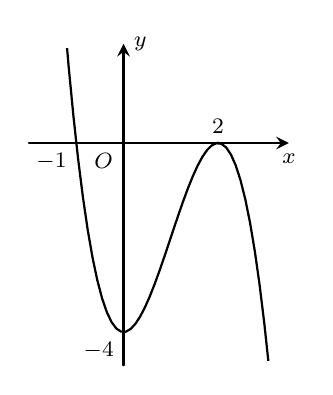
\begin{tikzpicture}[scale=0.6,>=stealth, font=\footnotesize, line join=round, line cap=round]
			\draw[->,line width=1pt] (-2,0)--(0,0) node[below left]{$O$}--(3.5,0) node[below]{$x$};
			\draw[->,line width=1pt] (0,-4.7)--(0,2.1) node[right]{$y$};
			\clip (-2,2) rectangle (3.1,-4.6);
			\draw[thick, samples=100] plot(\x,{-1*(\x)^3+3*(\x)^2-4});
			\fill[black] (0,-4)node[below left]{$-4$}circle(1pt)
			(2,0)node[above]{$2$}circle(1pt)
			(-1,0)node[below left]{$-1$}circle(1pt)
			;
		\end{tikzpicture}}
	\loigiai{
		Ta có $\lim\limits_{x \to+\infty}y=-\infty \Rightarrow a<0$ nên ta loại phương án $y=x^3-3x^2+4$ và $y=x^3-3x^2-4$.\\
		Đồ thị hàm số qua điểm $M(2 ; 0)$ nên ta chọn đáp án $y=-x^3+3x^2-4$.}
\end{ex}

\begin{ex}%[2D1V5-8]
	\immini
	{
		Cho một tấm gỗ hình vuông cạnh $200$ (cm). Người ta cắt một tấm gỗ có hình một tam giác vuông $ABC$ từ tấm gỗ hình vuông đã cho như hình vẽ sau. Biết $AB=x\,(\mathrm{cm})(0<x<60)$ là một cạnh góc vuông của tam giác $ABC$ và tổng độ dài cạnh góc vuông $AB$ với cạnh huyền $B C$ bằng $120$ (cm). Tìm $x$ để tam giác $ABC$ có diện tích lớn nhất.
		\choice
		{\True $x=40$ (cm)}
		{$x=50$ (cm)}
		{$x=30$ (cm)}
		{$x=20$ (cm)}
	}
	{
		\begin{tikzpicture}[scale=1,font=\footnotesize,line join=round,line cap=round,>=stealth]
			\path
			(0,0) coordinate (A)
			(5,5) coordinate (E)
			(0,1) coordinate (B)
			(4,0) coordinate (C)
			(5,0) coordinate (F)
			(0,5)coordinate (D)
			;
			\draw (B)--(D)--(E)--(F)--(C);
			\draw[dashed] (A)--(B)--(C)node[midway,above]{$120-x$}--cycle;
			\foreach \p/\q in {A/-135,B/180,C/-90}
			\fill[black] (\p) circle (1.0pt) ($(\p)+(\q:2.5mm)$) node{$\p$};
			\node at ($(A)!0.5!(B)$)[left]{$x$};
			\node at ($(D)!0.5!(E)$)[above]{$200$};
		\end{tikzpicture}
	}
	\loigiai{
	Độ dài cạnh huyền $B C=120-x$.\\
	Khi đó độ dài cạnh $A C=\sqrt{B C^{2}-A B^{2}}=\sqrt{(120-x)^{2}-x^{2}}=\sqrt{14400-240 x}$.\\
	Diện tích tam giác $ABC$ là $S=\dfrac{1}{2} A B \cdot A C=\dfrac{1}{2} x \sqrt{14400-240 x}\left(\mathrm{~cm}^{2}\right)$\\
	Xét hàm số $f(x)=x \sqrt{14400-240 x}$ với $0<x<60$.\\
	Ta có $f'(x)=\sqrt{14400-240 x}-\dfrac{120 x}{\sqrt{14400-240 x}}=\dfrac{14400-360 x}{\sqrt{14400-240 x}}$;\\
	$f'(x)=0 \Leftrightarrow x=40 \in(0 ; 60)$\\
	Bảng biến thiên
	\begin{center}
		
\begin{tikzpicture}
			\tkzTabInit[nocadre=false,lgt=1.2,espcl=2.5,deltacl=0.6]
			{$x$ /0.6, $f'(x)$ /0.6, $f(x)$ /2.5}
			{$0$,$40$,$60$}
			\tkzTabLine{,+,$0$,-,}
			\tkzTabVar{-/,+/,-/}
		\end{tikzpicture}
	\end{center}
	Vậy tam giác $ABC$ có diện tích lớn nhất khi $AB=40$ (cm).
	}
\end{ex}

\begin{ex}%[KNTT]giảng 12 New-4in1, Toàn Phan]%[2D1H5-8]KNTT
	Khi bỏ qua sức cản của không khí, độ cao (mét) của một vật được phóng thẳng đứng lên trên từ điểm cách mặt đất $2$ m với vận tốc ban đầu $24{,}5$ m/s là $h(t)=2+24{,}5t-4{,}9t^2$ (theo Vật lí đại cương, NXB Giáo dục Việt Nam, $2016$). Tìm vận tốc của vật sau $2$ giây.
	\choice
	{\True $4{,}9$}
	{$2{,}4$}
	{$3{,}5$}
	{$5{,}2$}
	\loigiai{
	Theo ý nghĩa cơ học của đạo hàm, vận tốc của vật là $v=h'(t)=24{,}5-9{,}8t$ m/s.\\
	Do đó, vận tốc của vật sau $2$ giây là $v(2)=24{,}5-9{,}8\cdot 2=4{,}9$ m/s.
	}
\end{ex}

\begin{ex}%[De-chuan-hoa-so-1]%[Mui Doan]%[2D1H5-8]
	Độ giảm huyết áp của một bệnh nhân được cho bởi công thức $G(x)=0{,}035x^2(15-x)$, trong đó $x$ là liều lượng thuốc được tiêm cho bệnh nhân ($x$ được tính bằng miligam). Liều lượng thuốc cần tiêm (đơn vị miligam) cho bệnh nhân để huyết áp giảm nhiều nhất là
	\choice
	{$x=8$}
	{\True $x=10$}
	{$x=15$}
	{$x=7$}
	\loigiai{
	Điều kiện $x\in[0;15]$ (vì độ giảm huyết áp không thể là số âm).\\
	Có $G'(x)=0{,}035\left[2x(15-x)-x^2\right]=0{,}105x(10-x)=0\Leftrightarrow\hoac{&x=0\\&x=10.}$ \\
	Ta có $G(0)=0$; $G(10)=\dfrac{35}{2}$; $G(15)=0$.\\
	Bảng biến thiên
	\begin{center}
		
\begin{tikzpicture}
			\tkzTab
			[lgt=1.5,espcl=3]
			{$x$/0.8, $G'(x)$/0.8, $G(x)$/2.5}
			{$0$, $10$, $15$}
			{,+,0,-,}
			{-/$0$ , +/ $\dfrac{35}{2}$ , -/$0$} %
		\end{tikzpicture}
	\end{center}
	Vậy huyết áp bệnh nhân giảm nhiều nhất khi tiêm cho bệnh nhân liều $x=10$ miligam.}
\end{ex}

\begin{ex}%[2H2N1-1]%[CD - Lớp 12 - Ôn tập cuối học kì 1 - Đề 5]%[Đoàn Thị Lý]
	Cho hình hộp $ABCD.A'B'C' D'$. Vectơ nào dưới đây cùng phương với vectơ $\overrightarrow{AB}$?
	\choice
	{\True $\overrightarrow{CD}$}
	{$\overrightarrow{B'C'}$}
	{$\overrightarrow{AD}$}
	{$\overrightarrow{AC'}$}
	\loigiai{
		\immini{
			Vectơ cùng phương với $\overrightarrow{AB}$ là $\overrightarrow{CD}$, vì hai vectơ này có giá song song với nhau.}
		{
			\begin{tikzpicture}[line join = round, line cap = round,>=stealth,scale=1]
				\def\a{3}
				\def\b{1}
				\def\g{30}
				\def\h{2}
				\path
				(0:0) coordinate (A)--++(\g:\b) coordinate (B)--++(0:\a) coordinate (C)--++(\g-180:\b) coordinate (D)
				\foreach \x in {A,B,C,D}{
						($(\x)+(70:\h)$) coordinate (\x')}
				;
				\foreach \x/\g in {A/180,B/150,C/0,D/-30,A'/180,B'/150,C'/0,D'/-30}
				\fill[black](\x) circle (1pt)
				($(\x)+(\g:3mm)$) node{$\x$};
				\draw[dashed] (B')--(B)--(A)
				(B)--(C);
				\draw
				(A)--(D)--(D')--(A')--cycle
				(A')--(B')--(C')--(D')
				(D)--(C)--(C')
				;
			\end{tikzpicture}
		}
	}
\end{ex}

\begin{ex}%[Dự án EX-Ôn tập 2025, Đào-V- Thuỷ]%[2H2N1-2]
	Cho tứ diện $ABCD$. Lấy $G$ là trọng tâm của tam giác $ABC$. Phát biểu nào sau đây là \textbf{sai}?
	\choice
	{$\vec{GA}+ \vec{GB}+ \vec{GC}= \vec{0}$}
	{\True $\vec{GA}+ \vec{GB}+ \vec{GC}+ \vec{GD}= \vec{0}$}
	{$\vec{GD}- \vec{GA}= \vec{AD}$}
	{$\vec{DA}+ \vec{DB}+ \vec{DC}= 3\vec{DG}$}
	\loigiai
	{
		Theo tính chất, vì $G$ là trọng tâm $\triangle ABC$ nên $\vec{GA}+ \vec{GB}+ \vec{GC}= \vec{0}$.\\
		Do đó $\vec{GA}+ \vec{GB}+ \vec{GC}+ \vec{GD}= \vec{GD} \neq \vec{0}$.
	}
\end{ex}

\begin{ex}%[2H2N1-3]
	Cho hình chóp $S.ABCD$ có $ABCD$ là hình vuông cạnh $ a $. Cạnh bên $ SA $ vuông góc với mặt đáy $ (ABCD) $ và $ SA=a\sqrt{3} $. Tích vô hướng của hai véc-tơ $\overrightarrow{CB} $ và $\overrightarrow{DS}$ bằng
	\choice
	{$a^2$}
	{$2a^2$}
	{$a^2\sqrt{2}$}
	{\True$a^2\sqrt{3}$}
	\loigiai{
		\immini
		{
			Do  $ABCD$ là hình vuông nên  $\overrightarrow{CB} =\overrightarrow{DA}.$\\
			$\Rightarrow \left (\overrightarrow{CB},\overrightarrow{DS}\right )=\left (\overrightarrow{DA},\overrightarrow{DS}\right )=\widehat{ADS}$.\\
			Xét $ \triangle ASD $ vuông tại $ A $ có $SA=a\sqrt{3}$, $AD=a$, $SD=2a$.\\
			$ \tan \widehat{ASD}=\dfrac{SA}{AD}=\sqrt{3} \Rightarrow \widehat{ASD}=60^\circ$.\\
			Vậy $\overrightarrow{CB}\cdot\overrightarrow{DS}=\overrightarrow{DA}\cdot\overrightarrow{DS}=a\cdot 2a\cdot\cos60^\circ=a^2\sqrt{3}$.
		}
		{
			\begin{tikzpicture}[scale=0.5, font=\normalsize, line join=round, line cap=round, >=stealth]
				\path
				(0,0) coordinate (A)
				(-2,-2) coordinate (B)
				(3,-2) coordinate (C)
				(5,0) coordinate (D)
				(0,5)coordinate (S)
				;
				\begin{scope}
					\clip (S)--(D)--(A);
					\draw[fill=magenta!20] (D) circle(0.7cm);
				\end{scope}

				\draw (B)--(C)--(D) (S)--(B)(S)--(C)(S)--(D)
				pic [draw=red,fill=yellow!30,angle radius=3mm] {right angle = S--A--D};
				\draw[dashed] (A)--(B) (A)--(C) (A)--(D) (S)--(A);

				\foreach \p/\r in {A/120,B/-120,C/-60,D/0,S/90}
				\draw[fill=black] (\p) circle (0.7pt) node[shift={(\r:3mm)}]{$\p$};
			\end{tikzpicture}
		}

	}
\end{ex}

\begin{ex}%[2H2H1-2]
	Cho hình hộp $ABCD.A_{1} B_{1} C_{1} D_{1} $. Trong các khẳng định sau, khẳng định nào \textbf{sai}?
	\choice
	{\True $\overrightarrow{AC_{1} }+\overrightarrow{A_{1} C}=2\overrightarrow{AC}$}
	{$\overrightarrow{AC_{1} }+\overrightarrow{CA_{1} }+2\overrightarrow{C_{1} C}=\overrightarrow{0}$}
	{$\overrightarrow{AC_{1} }+\overrightarrow{A_{1} C}=\overrightarrow{AA_{1} }$}
	{$\overrightarrow{CA_{1} }+\overrightarrow{AC}=\overrightarrow{CC_{1} }$}
	\loigiai{
		\immini{
			\begin{itemize}
				\item Gọi $O$ là tâm của hình hộp $ABCD.A_{1} B_{1} C_{1} D_{1} $.
				\item Vận dụng công thức trung điểm để kiểm tra.
			\end{itemize}
		}{
			\begin{tikzpicture}[scale=0.5, font=\footnotesize,line join=round, line cap=round, >=stealth]
				\coordinate (A) at (0,0);
				\coordinate (B) at (-2,-2);
				\coordinate (D) at (6,0);
				\coordinate (C) at ($(B)+(D)-(A)$);
				\coordinate (C') at ($(C)+(0,4)$);
				\coordinate (O) at ($(A)!0.5!(C')$);
				\foreach \i in {A,B,C,D}{\coordinate (\i_1) at ($(\i)+(0,4)$);}
				\draw (A_1)--(B_1)--(C_1)--(D_1)--cycle;
				\draw (B)--(B_1) (C)--(C_1) (D)--(D_1)  (B)--(C)--(D);
				\draw[dashed,thin](B)--(A)--(A_1) (A)--(D);
				\draw[->,dashed](A) -- (C);
				\draw[->,dashed](A) -- (C_1);
				\draw[->,dashed](A_1) -- (C);
				\draw[->,dashed](A_1) -- (O);
				\foreach \i/\g in {A_1/90,B_1/90,C_1/90,D_1/90,A/-90,B/-90,C/-90,D/-90,O/-90}{\draw[fill=blue](\i) circle (1.5pt) ($(\i)+(\g:5mm)$) node[scale=1]{$\i$};}
			\end{tikzpicture}
		}
	}
\end{ex}

\begin{ex}%[De-chuan-hoa-so-22]%[Phạm Tuấn]%[2H2H1-3]
	Cho tứ diện đều $ABCD$ có tất cả các cạnh bằng  $6$. Tính tích vô hướng $\overrightarrow{AB} \cdot \overrightarrow{CD}$.
	\choice
	{\True $0$}
	{$-12$}
	{$12$}
	{$36$}
	\loigiai{
		\immini{
			Ta có
			\begin{align*}
				\overrightarrow{AB} \cdot \overrightarrow{CD} & = \overrightarrow{AB} \cdot (\overrightarrow{AD} - \overrightarrow{AC})                            \\
				                                              & =  \overrightarrow{AB} \cdot  \overrightarrow{AD} - \overrightarrow{AB} \cdot  \overrightarrow{AC} \\
				                                              & =  6 \cdot 6 \cdot \cos 60^\circ - 6 \cdot 6 \cdot \cos 60^\circ  =0.
			\end{align*}
		}
		{
			\begin{tikzpicture}
				\path
				(1,3) coordinate (A)
				(0,0) coordinate (B)
				(0.8,-1.2) coordinate (C)
				(4.5,0) coordinate (D)
				;
				\draw (A)--(B)--(C)--(A)--(D)--(C);
				\draw [dashed] (B)--(D);
				\foreach \x/\g in {A/90,B/180,C/-90,D/0}
				\fill[black] (\x) circle(1.1pt) + (\g:3.5mm) node {$\x$};
			\end{tikzpicture}
		}
	}
\end{ex}

\begin{ex}%[De-chuan-hoa-so-20]%[Ninh Tiến Nam]%[2H2H1-1]
	Trong không gian $Oxyz$, cho ba điểm $A(1;2;0),B(5;3;-1),C(2;3;-4)$. Tọa độ tâm $K$ của đường tròn nội tiếp $\triangle ABC$ là
	\choice
	{ $K\left(3;\dfrac{3}{5},-\dfrac{1}{2}\right)$}
	{ $K\left(\dfrac{7}{2};3;-\dfrac{5}{3}\right)$}
	{$K\left(\dfrac{8}{3};\dfrac{8}{3};\dfrac{5}{3}\right)$}
	{\True  $K\left(\dfrac{8}{3};\dfrac{8}{3};-\dfrac{5}{3}\right)$}
	\loigiai{
		Ta có $AB=3\sqrt{2}; BC=3\sqrt{2};CA=3\sqrt{2}$.\\
		Do $\triangle  ABC$ là tam giác đều nên  tâm đường tròn nội tiếp $K$ của $\triangle ABC$ đồng thời là trọng tâm của tam giác $\triangle ABC$, ta có

		\[\heva{
				&x_K = \dfrac{1+5+2}{3}=\dfrac{8}{3} \\
				&y_K = \dfrac{2+3+3}{3}=\dfrac{8}{3} \\
				&z_K = \dfrac{0+(-1)+(-4)}{3}=\dfrac{-5}{3}.}\]



		Vây $K=\left(\dfrac{8}{3};\dfrac{8}{3};-\dfrac{5}{3}\right)$.
	}
\end{ex}

\begin{ex}%[2H2V1-3] 8
	Trong các mệnh đề sau đây, mệnh đề nào \textbf{sai}?
	\choice
	{Vì $I$ là trung điểm đoạn $AB$ nên từ $O$ bất kì ta có: $\overrightarrow{OI}=\dfrac{1}{2}( \overrightarrow{OA}+\overrightarrow{OB} )$}
	{\True Vì $\overrightarrow{AB}+\overrightarrow{BC}+\overrightarrow{CD}+\overrightarrow{DA}=\overrightarrow{0}$ nên bốn điểm $A,B,C,D$ đồng phẳng}
	{Vì $\overrightarrow{NM}+\overrightarrow{NP}=\overrightarrow{0}$ nên $N$ là trung điểm đoạn $NP$}
	{Từ hệ thức $\overrightarrow{AB}=2\overrightarrow{AC}-8\overrightarrow{AD}$ ta suy ra ba vectơ $\overrightarrow{AB},\,\overrightarrow{AC},\,\overrightarrow{AD}$ đồng phẳng.
	}
	\loigiai{
		Do $\overrightarrow{AB}+\overrightarrow{BC}+\overrightarrow{CD}+\overrightarrow{DA}=\overrightarrow{0}$ đúng với mọi điểm $A,B,C,D$ nên câu B sai}
\end{ex}

\begin{ex}%[Lê Vũ Hải]%[2H2N2-2]
	Cho tam giác $ABC$ với $A(1;-2;0)$, $B(2;1;-2)$, $C(0;3;4)$. Tìm tọa độ điểm $D$ để $ABDC$ là hình bình hành.
	\choice
	{$(1;0;-6)$}
	{$(-1;0;6)$}
	{\True $(1;6;2)$}
	{$(1;6;-2)$}
	\loigiai{
		Gọi $D(x;y;z)$. Để $ABDC$ là hình bình hành thì $\vec{AB}=\vec{CD} \Leftrightarrow \heva{& 1=x-0 \\& 3=y-3\\& -2=z-4} \Leftrightarrow \heva{& x=1\\&y=6 \\&z=2.}$\\
		Vậy $D(1;6;2)$.
	}
\end{ex}

\begin{ex}%[12-MH-1-MH2025]%[MH-2025, Mã/Tên TV biên soạn]%[2H2N2-1]
	Trong không gian $Oxyz$, tọa độ của vectơ $\vec{k}$ là
	\choice
	{$(1;1;1)$}
	{$(1;0;0)$}
	{$(0;1;0)$}
	{\True $(0;0;1)$}
	\loigiai{
		Trong không gian $Oxyz$, tọa độ của vectơ $\vec{k}$ là $(0;0;1)$.}
\end{ex}

\begin{ex}%[VN-MT-7, Lê Minh Thiện Anh]%[2H2N2-4]
	Trong không gian $Oxyz$, cho hai vectơ $\overrightarrow{a}=(4;-3;-1)$ và $\overrightarrow{b}=\overrightarrow{i}+2\overrightarrow{j}+\overrightarrow{k}$. Tìm tọa độ của vectơ $2\overrightarrow{a}+3\overrightarrow{b}$.
	\choice
	{\True $(11;0;1)$}
	{$(5;-1;0)$}
	{$(11;0;-1)$}
	{$(5;-1;-1)$}
	\loigiai{
		Ta có $2\overrightarrow{a}=(8;-6;-2)$ và $\overrightarrow{b}=\overrightarrow{i}+2\overrightarrow{j}+\overrightarrow{k}\Rightarrow \overrightarrow{b}=(1;2;1)\Rightarrow 3\overrightarrow{b}=(3;6;3)$.\\
		Do đó $2\overrightarrow{a}+3\overrightarrow{b}=(8+3;-6+6;-2+3)=(11;0;1)$.
	}
\end{ex}

\begin{ex}%[2-H2B2-SO-6-2425]%[VN-MT-7, VM035]%[2H2H2-1]
	Trong không gian với hệ tọa độ $Oxyz$, cho vectơ $\overrightarrow{A O}=3\left(\overrightarrow{i}+4 \overrightarrow{j}\right)-2 \overrightarrow{k}+5\overrightarrow{j}$. Tọa độ của điểm $A$ là
	\choice
	{$(3;17;-2)$}
	{\True $(-3;-17;2)$}
	{$(3;-2;5)$}
	{$(3;5;-2)$}
	\loigiai{Ta có $\overrightarrow{A O}=3\left(\overrightarrow{i}+4 \overrightarrow{j}\right)-2 \overrightarrow{k}+5 \overrightarrow{j}=3 \overrightarrow{i}+12 \overrightarrow{j}-2 \overrightarrow{k}+5 \overrightarrow{j}=3 \overrightarrow{i}+17 \overrightarrow{j}-2 \overrightarrow{k}$.\\
		Suy ra $\overrightarrow{OA}=-3 \overrightarrow{i}-17 \overrightarrow{j}+2 \overrightarrow{k}$ nên $A(-3;-17;2)$.}
\end{ex}

\begin{ex}%[De-chuan-hoa-so-20]%[Ninh Tiến Nam]%[Thi Thử lần 1-Nguyễn Trãi-Hải Dương, 2022]%[Hoàng Trọng Tấn, dự án(12EX-3)]%[2H2H2-4]
	Trong không gian $Oxyz$, cho $A(0;-1;-1)$, $B(-2;1;1)$, $C(-1;3;0)$, $D(1;1;1)$. Tính cô-sin của góc giữa hai đường thẳng $AB$ và $CD$.
	\choice
	{\True $\dfrac{\sqrt{3}}{3}$}
	{$-\dfrac{\sqrt{6}}{3}$}
	{$-\dfrac{\sqrt{3}}{3}$}
	{$\dfrac{\sqrt{6}}{2}$}
	\loigiai{
		Ta có $\overrightarrow{A B}=(-2 ; 2 ; 2)$, $\overrightarrow{C D}=(2 ;-2 ; 1)$.
		\\
		Suy ra
		$\cos \widehat{(A B, C D)}=\left|\cos (\overrightarrow{A B}, \overrightarrow{C D})\right|=\dfrac{\left|\overrightarrow{A B} \cdot \overrightarrow{C D}\right|}{A B \cdot C D}=\dfrac{6}{2 \sqrt{3} \cdot 3}=\dfrac{1}{\sqrt{3}}$.
	}
\end{ex}

\begin{ex}%[2H2V2-6]
	Cho hình hộp chữ nhật $ABCD.A'B'C'D'$ có các kích thước $AB=4$, $AD=3$, $AA'=5$. Gọi $G$ là trọng tâm của tam giác $ACB'$. Độ dài $BG$ là:
	\choice
	{$BG=\dfrac{\sqrt{2}}{3}$}
	{$BG=\dfrac{2\sqrt{5}}{3}$}
	{$BG=\dfrac{5\sqrt{2}}{2}$}
	{\True $BG=\dfrac{5\sqrt{2}}{3}$}
	\loigiai{
		Chọn hệ trục tọa độ như hình vẽ.
		\begin{center}\begin{tikzpicture}[>=stealth,line join=round,line width=1pt,line cap=round]
				\draw[black,scale=2.5] (0,0)coordinate(A)  (-120:1)coordinate(D)--($(1.5,0)-(A)+(D)$)coordinate(C)--(1.5,0)coordinate(B);
				\draw[dashed,line width=1pt,black,scale=2.5] (D)--(A)--(B) ($(A)+(90:1)$)coordinate(A')--(A);
				\draw (D)--($(A')-(A)+(D)$)coordinate(D')--($(A')-(A)+(C)$)coordinate(C')--($(A')-(A)+(B)$)coordinate(B')--(A') (C)--(C') (D')--(A') (B')--(B);
				\path[scale=2.5] pic[angle radius=5,draw=blue,angle eccentricity=1.5] {right angle = B--A--A'};
				\draw[->, red] (B)--($1.25*(B)-0.25*(A)$)coordinate(Y)node[above]{$y$};
				\draw[->, red] (D)--($1.25*(D)-0.25*(A)$)coordinate(X)node[left]{$x$};
				\draw[->, red] (A')--($1.25*(A')-0.25*(A)$)coordinate(Z)node[right]{$z$};
				\foreach \diem/\vitrin in {A'/left,A/left,D/left,C/below right,B/above right,D'/left, C'/above,B'/above right}\fill (\diem)circle(1.5pt)node[\vitrin]{$\diem$};
			\end{tikzpicture}\end{center}
		Ta có $A(0;0;0)$, $C(4;3;0)$, $B'(4;0;5)$, $B(4;0;0)$.\\
		$G$ là trọng tâm của tam giác $ACB'$, suy ra $G\left(\dfrac{8}{3};1;\dfrac{5}{3}\right)$.\\
		Độ dài $BG$ là $BG=\sqrt{\left(\dfrac{8}{3}-4\right)^2+\left(1-0\right)^2+\left(\dfrac{5}{3}-0\right)^2}=\dfrac{5\sqrt{2}}{3}$.
	}
\end{ex}

\begin{ex}%[2D3N1-1]%[CD - Lớp 12 - Ôn tập cuối học kì 1 - Đề 04]%[Phạm Lương]
	Thời gian truy cập Internet mỗi buổi tối của một số học sinh được cho trong bảng sau
	\begin{center}
		\begin{tabular}{|c|c|c|c|c|c|}
			\hline
			Thời gian (phút) & $[9{,}5;12{,}5)$ & $[12{,}5;15{,}5)$ & $[15{,}5;18{,}5)$ & $[18{,}5;21{,}5)$ & $[21{,}5;24{,}5)$ \\ \hline
			Số học sinh      & $3$              & $12$              & $15$              & $24$              & $2$               \\ \hline
		\end{tabular}
	\end{center}
	Tần số tích lũy của nhóm $[18{,}5; 21{,}5)$ là
	\choice
	{$24$}
	{$39$}
	{$30$}
	{\True $54$}
	\loigiai
	{Tần số tích lũy của nhóm $[18{,}5; 21{5})$ là $3+12+15+24 = 54$.
	}
\end{ex}

\begin{ex}%[2D3H1-2]%[KNTT - Lớp 12 - Ôn tập cuối học kì 1 - Đề 6]%[Long]
	Thống kê chiều cao học sinh hai lớp $11A$ và $11B$ của một trường THPT được bảng số liệu sau
	\begin{center}
		\begin{tabular}{|c|c|c|c|c|c|c|}
			\hline
			Chiều cao (cm) & {$[145; 150)$} & {$[150; 155)$} & {$[155; 160)$} & {$[160; 165)$} & {$[165; 170)$} & {$[170; 175]$} \\
			\hline
			Lớp $11A$      & $0$            & $4$            & $10$           & $16$           & $8$            & $2$            \\
			\hline
			Lớp $11B$      & $1$            & $5$            & $8$            & $15$           & $13$           & $3$            \\
			\hline
		\end{tabular}
	\end{center}
	Theo bảng trên, kết luận nào sau là đúng?
	\choice
	{Khoảng biến thiên về chiều cao học sinh lớp $11A$ bằng $30$}
	{Khoảng biến thiên về chiều cao học sinh lớp $11A$ lớn hơn lớp $11B$}
	{Khoảng biến thiên về chiều cao học sinh của hai lớp $11A$ và $11B$ bằng nhau}
	{\True Chiều cao học sinh lớp $11B$ phân tán hơn chiều cao học sinh lớp $11A$}
	\loigiai{
		Khoảng biến thiên về chiều cao học sinh lớp $11A$ là $R_A=175-150=25$.\\
		Khoảng biến thiên về chiều cao học sinh lớp $11B$ là $R_B=175-145=30$.\\
		Vậy chiều cao học sinh lớp $11B$ phân tán hơn chiều cao học sinh lớp $11A$, (do $R_B > R_A$).
	}
\end{ex}

\begin{ex}%[2-D3B2-SO-6-2425]%[VN-MT-7, Đỗ Nam]%[2D3H1-3]
	Mẫu số liệu ghép nhóm thống kê mức lương của một công ty (đơn vị: triệu đồng) được cho trong bảng dưới đây:
	\begin{center}
		\begin{tabular}{|l|c|c|c|c|c|c|}
			\hline
			Mức lương (triệu đồng) & $[6;8)$ & $[8;10)$ & $[10;12)$ & $[12;14)$ & $[14;16)$ &        \\
			\hline
			Tần số                 & $6$     & $14$     & $18$      & $10$      & $2$       & $n=50$ \\
			\hline
		\end{tabular}
	\end{center}
	Tìm khoảng tứ phân vị của mẫu số liệu ghép nhóm (làm tròn đến hàng phần trăm).
	\choice
	{\True $3{,}02$}
	{$3{,}15$}
	{$3{,}34$}
	{$2{,}96$}

	\loigiai{
		\begin{itemize}
			\item Tìm tứ phân vị thứ nhất.\\
			      Cỡ mẫu $n=50$. \\
			      Gọi $x_1$, $x_2$, $x_3$, $\ldots$, $x_{50}$ là mẫu số liệu gốc sắp xếp theo thứ tự không giảm gồm mức lương của một công ty. \\
			      Ta có $x_1$, $\ldots$, $x_6$ $\in [6;8)$; $x_{7}$, $\ldots$, $x_{20}$ $\in [8;10)$; $x_{21}$, $\ldots$, $x_{38}$ $\in [10;12)$; $x_{39}$, $\ldots$, $x_{48}$ $\in [12;14)$; $x_{48}$, $\ldots$, $x_{50}$ $\in [14;16)$. \\
			      Tứ phân vị thứ nhất của mẫu số liệu gốc là $\dfrac{1}{2} (x_{12} + x_{13}) \in [8;10)$. Do đó, tứ phân vị thứ nhất của mẫu số liệu ghép nhóm là
			      \[Q_1 = 8 +\dfrac{12{,}5-6}{14}\cdot 2 = \dfrac{125}{14}\ \text{(triệu đồng)}.\]
			\item Tìm tứ phân vị thứ ba.\\
			      Tứ phân vị thứ ba của mẫu số liệu gốc là $\dfrac{1}{2} (x_{37} + x_{38}) \in [10;12)$. Do đó, tứ phân vị thứ ba của mẫu số liệu ghép nhóm là
			      \[Q_3 = 10 + \dfrac{37{,}5-20}{18}\cdot 2 = \dfrac{215}{18}\,\text{(triệu đồng).}\]
			\item Khoảng tứ phân vị của mẫu số liệu ghép nhóm là
			      \[\Delta_{Q} = Q_3 - Q_1 = \dfrac{215}{18} - \dfrac{125}{14} \approx 3{,}02\,\text{(triệu đồng)}.\]
		\end{itemize}
	}
\end{ex}

\begin{ex}%[2D3H1-4]
	Cho bảng phân bố tần số sau
	\begin{center}
		\newcolumntype{P}[1]{>{\centering\arraybackslash}p{#1}}
		\begin{tabular}{|c|P{0.6in}|P{0.6in}|P{0.6in}|P{0.6in}|P{0.6in}|}
			\hline
			Giá trị & $x_1$ & $x_2$ & $x_3$ & $x_4$  & $x_5$ \\
			\hline
			Tần số  & 3     & 5     & $n+6$ & $20-n$ & 9     \\
			\hline
		\end{tabular}
	\end{center}
	Trong đó $ n $ là số tự nhiên và giá trị $x_4 $ là mốt duy nhất của bảng số liệu thống kê đã cho. Có bao nhiêu giá trị $n$ thỏa mãn yêu cầu?
	\choice
	{\True$7$}
	{$6$}
	{$5$}
	{$4$}
	\loigiai{
		Từ giả thiết $x_4$ là mốt duy nhất của bảng số liệu thống kê đã cho nên ta có
		\[\heva{& 20-n>9 \\   & 20-n>n+6}\Leftrightarrow \heva{ & n<11 \\   & n<7}\Leftrightarrow n<7.\]
		Vì $n$ là số tự nhiên nên các giá trị $n$ thỏa mãn là $0\le n<7$.
	}
\end{ex}

\begin{ex}%[2D3H2-1]%[Du-An-Ngan-Hang-Cau-Hoi-2024-K12]
	Khẳng định nào sau đây là đúng?
	\choice
	{Phương sai và độ lệch chuẩn càng cao thì độ phân tán của các số liệu thống kê càng thấp}
	{\True Phương sai và độ lệch chuẩn càng nhỏ thì độ phân tán của các số liệu thống kê càng nhỏ}
	{Phương sai và độ lệch chuẩn càng nhỏ thì độ phân tán của các số liệu thống kê càng lớn}
	{Phương sai và độ lệch chuẩn càng lớn thì độ phân tán của các số liệu thống kê càng nhỏ}
	\loigiai{Mẫu số liệu nào có độ phân tán lớn hơn thì phương sai và độ lệch chuẩn càng lớn.}
\end{ex}

\begin{ex}%[Mức độ 2]Giảng Toán 12 Sách mới 4in1, Quan Ón]%[2D3H2-2]
	Phương sai của mẫu số liệu cho bởi \textit{Bảng 1} là
	\choice
	{$ S^2 = \dfrac{8}{15} - \left(\dfrac{7}{15} \right)^2 $}
	{$ S^2 = \dfrac{233}{15} - \left(\dfrac{50}{15} \right)^2 $}
	{$ S^2 = \dfrac{8}{15} - \left(\dfrac{57}{15} \right)^2 $}
	{\True $ S^2 = \dfrac{233}{15} - \left(\dfrac{57}{15} \right)^2 $}
	\loigiai{
		Cỡ mẫu $n = 15$.
		\begin{center}
			\begin{tabular}{|l|c|c|c|c|c|}
				\hline
				\textbf{Nhóm}             & $[1{,}5; 2{,}5)$ & $ [2{,}5; 3{,}5)$ & $ [3{,}5; 4{,}5)$ & $ [4{,}5; 5{,}5)$ & $ [5{,}5; 6{,}5)$ \\
				\hline
				\textbf{Giá trị đại diện} & $2$              & $3$               & $4$               & $5$               & $6$               \\
				\hline
				\textbf{Tần số}           & $2$              & $3$               & $7$               & $2$               & $1$               \\
				\hline
			\end{tabular}
		\end{center}
		\noindent
		Giá trị trung bình của mẫu số liệu trên là
		\[\overline{x} = \dfrac{2\cdot 2 + 3\cdot 3 + 7\cdot 4 + 2\cdot 5 + 1\cdot 6}{15} = \dfrac{57}{15}.\]
		Phương sai của mẫu số liệu trên là
		\[S^2 = \dfrac{1}{15}\left(2\cdot 2^2 + 3\cdot 3^2 + 7\cdot 4^2 + 2\cdot 5^2 + 1\cdot 6^2\right) - \left(\dfrac{57}{15}\right)^2 = \dfrac{233}{15} - \left(\dfrac{57}{15}\right)^2.\]
	}
\end{ex}
\Closesolutionfile{ans}
\TL
\begin{bt}%[2D3H2-2] %[To11-Dot16-Chuong3-Ontapchuong-CD-De3]%[Hector Tran]
	Bảng dưới đây biểu diễn mẫu số liệu ghép nhóm về chiều cao (đơn vị: centimet) của $43$ học sinh trong một lớp học khối $11$ của một trường phổ thông
	\begin{center}
		\begin{tabular}{|c|c|c|}
			\hline
			Nhóm        & Giá trị đại diện & Tần số \\
			\hline
			$[150;155)$ & $152{,}5$        & $5$    \\
			\hline
			$[155;160)$ & $157{,}5$        & $10$   \\
			\hline
			$[160;165)$ & $162{,}5$        & $12$   \\
			\hline
			$[165;170)$ & $167{,}5$        & $9$    \\
			\hline
			$[170;175)$ & $172{,}5$        & $4$    \\
			\hline
			$[175;180)$ & $177{,}5$        & $3$    \\
			\hline
			            &                  & $n=43$ \\
			\hline
		\end{tabular}
	\end{center}
	Phương sai của mẫu số liệu ghép nhóm trên bằng bao nhiêu \textit{(làm tròn đến hàng phần mười)}?
	\loigiai
	{
		\begin{itemize}
			\item Số trung bình cộng của mẫu số liệu ghép nhóm trên là\\
			      $\overline{x}=\dfrac{5\cdot 152{,}5+10\cdot 157{,}5+12\cdot 162{,}5+9\cdot 167{,}5+4\cdot 172{,}5+3\cdot 177{,}5}{43} =\dfrac {14\,035}{86}$ (cm).
			\item Phương sai của mẫu số liệu ghép nhóm trên là\\
			      $s^2=\dfrac{1}{43} \left[5\cdot 152{,}5^2+10\cdot 157{,}5^2+12\cdot 162{,}5^2+9\cdot 167{,}5^2+4\cdot 172{,}5^2+3\cdot 177{,}5^2\right]-\left(\dfrac {14\,035}{86}\right)^2\approx 47{,}2$.
		\end{itemize}
	}
\end{bt}

\begin{bt}%[2D1H5-8]
	Trong một nhà hàng, mỗi tuần để chế biến $x$ phần ăn ($x$ lấy giá trị trong khoảng từ $30$ đến $120$) thì chi phí trung bình (đơn vị: nghìn đồng) của một phần ăn được cho bởi công thức:
	\[C(x)=2 x-230+\dfrac{7200}{x}.\]
	Tìm số phần ăn sao cho chi phí trung bình của một phần ăn là thấp nhất.
	\loigiai{
		\begin{itemize}
			\item Ta có $C'(x)=2-\dfrac{7200}{x^2}=0\Rightarrow \hoac{& x=60& (\text{nhận})\\ & x=-60&(\text{loại}).}$
			\item Bảng biến thiên
			      \begin{center}
				      
\begin{tikzpicture}
					      \tkzTabInit[nocadre=false,lgt=1.2,espcl=2.5,deltacl=0.6]
					      {$x$/0.6, $C’(x)$/0.6, $C(x)$/2}
					      {$30$, $60$, $120$}
					      \tkzTabLine{,-,0,+,}
					      \tkzTabVar{+/ , -/ $10$ , +/ }
				      \end{tikzpicture}
			      \end{center}
			\item Đồ thị của hàm số
			      \begin{center}
				      \begin{tikzpicture}[scale=0.2, font=\footnotesize, line join=round, line cap=round, >=stealth, xscale=0.4,yscale=0.4]
					      \draw[->] (-12,0) -- (125,0) node[above] {$x$};
					      \draw[->] (0,-8) -- (0,75) node[below right] {$y$};
					      \draw[smooth,domain=30:120,blue,thick] plot(\x,{7200/(\x)+2*(\x)-230});
					      \draw[dashed] (30,0)node[below]{$30$}--(30,70) (120,0)node[below]{$120$}--(120,70) (60,0)node[below]{$60$}|-(0,10)node[left]{$10$};
					      \fill (0,0) node[below left]{$O$}circle(14pt);
				      \end{tikzpicture}
			      \end{center}
		\end{itemize}
		Dựa vào đồ thị, số phần ăn $60$ thì chi phí trung bình của một phần ăn thấp nhất $10$ (nghìn đồng).
	}
\end{bt}

\begin{bt}%[Lê Vũ Hải]%[2H2V2-6]
	Với hệ trục $Oxyz$ sao cho $O$ nằm trên mặt nước, mặt phẳng $(Oxy)$ là mặt nước, trục $Oz$ hướng lên trên (đơn vị: mét). Một con chim bói cá đang ở vị trí cách mặt nước $2$ m, cách mặt phẳng $(Oxz)$ và $(Oyz)$ lần lượt là $3$ m và $1$ m phóng thẳng xuống vị trí con cá, biết con cá cách mặt nước $50$ cm, cách mặt phẳng $(Oxz)$, $(Oyz)$ lần lượt $75$ cm và $50$ cm. Tọa độ điểm $B(x;y;z)$ là khi chim bói cá vừa tiếp xúc với mặt nước, tính $x+y+z$.
	\shortans[]{$2{,}6$}
	\loigiai{
		\begin{center}
			\begin{tikzpicture}[line join = round, line cap = round, thick, font = \footnotesize, scale =1,>=stealth]
				\path
				(0,0) coordinate (O)++(0:4) coordinate (B)
				(O)++(90:2) coordinate (C)
				(O)++(-140:2) coordinate (A)
				($(A)+(B)-(O)$) coordinate (H)
				($(H)+(C)-(O)$) coordinate (M)
				($(O)!1.3!(A)$) coordinate (x) node[below]{$x$}
				($(O)!1.2!(B)$) coordinate (y) node[below]{$y$}
				($(O)!1.3!(C)$) coordinate (z) node[right]{$z$};
				\coordinate (C') at (0,-0.5);
				\coordinate (A') at ($(C')+(-140:1)$);
				\coordinate (Ca) at ($(A')+(1,0)$);
				\coordinate (Ca2) at ($(Ca)+(0,0.5)$);
				\coordinate (Cax) at ($(Ca2)+(-1,0)$);
				\coordinate (Cay) at ($(Ca2)+(40:1)$);
				\fill[color=cyan!30!white] (O)--(x)--($(x)+(y)$)--(y);
				\coordinate (N) at ($(Ca)!0.2!(M)$);
				\draw[dashed] (Ca)--(N) (Ca2)--(Cax)node[left]{0,5} (Ca2)--(Cay)node[above]{0,75};
				\draw (N)--(M);
				\draw (O)--(A) (O)--(B) (O)--(C);
				\draw[dashed] (C)--(M)--(H) (A)--(H)--(B) (Ca)--(Ca2)
				;
				\pic[draw,thin,angle radius=2mm] {right angle = M--C--O}
				pic[draw,thin,angle radius=2mm] {right angle = H--B--O}
				pic[draw,thin,angle radius=2mm] {right angle = H--A--O}
				;
				\draw[->] (A)--(x);
				\draw[->] (B)--(y);
				\draw[->] (C)--(z);
				\foreach \x/\g/\n in {A/150/1,H/-90/M',B/80/3,C/180/2,O/170/O,M/60/A,Ca/180/C,N/-70/B}
				\fill (\x) circle (1pt)
				+(\g:2mm) node[scale =1]{\n};
				\fill (Ca2) circle(1pt);
				\fill (Cax) circle(1pt);
				\fill (Cay) circle(1pt);
			\end{tikzpicture}
		\end{center}
		Ban đầu chim bói cá đang ở vị trí cách mặt nước $2$ m, cách mặt phẳng $(Oxz)$ và $(Oyz)$ lần lượt là $3$ m và $1$ m nên có tọa độ là $A(1;3;2)$. Vị trí của con cá cách mặt nước $50$ cm, cách mặt phẳng $(Oxz)$, $(Oyz)$ lần lượt $75$ cm và $50$ cm nên có tọa độ $C(0,5;0,75,-0,5)$.\\
		Theo đề bài, $B$ là vị trí mà con chim vừa tiếp xúc mặt nước, do đó ta có $B(x;y;0)$ do mặt nước là mặt phẳng $(Oxy)$.\\
		Ta có $\vec{AB}=(x-1;y-3;-2)$ và $\vec{AC}=(-0,5; -2,25; -2,5)$.\\
		Do ba điểm $A$, $B$, $C$ thẳng hàng nên hai véc-tơ $\vec{AB}$ và $\vec{AC}$ cùng phương, suy ra $\heva{&x-1 = k \cdot (-0,5)\\ & y-3=k\cdot (-2,25) \\& -2=k\cdot (-2,5)} \Leftrightarrow \heva{& k=0,8 \\& x=0,6 \\& y=1,2}$. \\
		Vậy $B(0,8; 0,6; 1,2)$, suy ra $x+y+z=2,6$.
	}
\end{bt}
\begin{ex}%[2D1V5-6]%[KNTT - Lớp 12 - Ôn tập cuối học kì 1 - Đề 1]%[Huỳnh Thanh Chí]
	\immini[thm]{Một hòn đảo nằm trong một hồ nước. Biết rằng đường cong tạo nên hòn đảo được mô hình hóa vào hệ trục tọa độ $Oxy$ là một phần của đồ thị hàm số bậc ba $f(x)$.\\
		Vị trí điểm cực đại là $(2; 5)$ với đơn vị của hệ trục là $100$ m và vị trí điểm cực tiểu là $(0; 1)$. Mặt đường chạy trên một đường thẳng có phương trình $y=36-9x$. Người ta muốn làm một cây cầu có dạng một đoạn thẳng nối từ hòn đảo ra mặt đường. Độ dài ngắn nhất của cây cầu bằng bao nhiêu mét? (Kết quả làm tròn đến hàng phần mười).}
	{\begin{tikzpicture}[scale=0.7,font=\footnotesize,line join=round,line cap=round,>=stealth]
			\draw[-stealth] (-0.2,0)--(6,0)node[below]{$x$};
			\draw[-stealth] (0,-1)--(0,5)node[left]{$y$};
			\draw (0,0) node [below right] {$O$};
			\draw[thick,smooth,samples=200] plot[domain=-0.2:3.2] (\x,{-(\x)^3+3*(\x)^2+1});
			\draw[thick,smooth,samples=200] plot[domain=3.33:4.1] (\x,{36-9*(\x)});
			\draw (3.5,5)node[right]{Mặt đường}
			(3.8,4) node[right]{$y=36-9x$}
			(0.7,2) node[right]{Hòn đảo} (1,5) node{$f(x)$}
			;
		\end{tikzpicture}}
	\shortans[]{$88{,}3$}
	\loigiai{Gọi hàm số bậc ba $y=f(x)=a x^3+b x^2+c x+d \Rightarrow f'(x)=3a x^2+2b x+c$.
		Vì đồ thị hàm số đi qua hai điểm $(0; 1) \Rightarrow d=1$.\\
		Vì đồ thị hàm số đi qua hai điểm $A(2; 5) \Rightarrow 8a+4b+2c+1=5$.\\
		Vì hàm số có hai điểm cực trị $x=0; x=2\Rightarrow\heva{&f'(0)=0\\
				&f'(2)=0} \Rightarrow\heva{&c=0\\
				&12a+4b=0.}$\\
		Suy ra $\heva{&a=-1\\
				&b=3} \Rightarrow f(x)=-x^3+3x^2+1$ và $f'(x)=-3x^2+6x$.\\
		Gọi $M\left(x_0; y_0\right)$, $x_0> 0$, là điểm nằm trên hòn đảo và nối với mặt đường và $(d)$ là tiếp tuyến của đồ thị hàm số song song với mặt đường. Suy ra $M$ là tiếp điểm của $(d)$ với $y=f(x)$.\\
		Đường thẳng $(d)\colon y=36-9x$ có hệ số góc $k=-9$.\\
		$\Rightarrow f'(x_0)=-9\Leftrightarrow-3x_0^2+6x_0=-9\Leftrightarrow\hoac{&x_0=3\\
				&x_0=-1} \Rightarrow M(3; 1)$.\\
		Độ dài cây cầu ngắn nhất bằng khoảng cách từ điểm $M$ đến đường thẳng $9x+y-36=0$.
		\[
			h=\dfrac{|9\cdot 3+1-36|}{\sqrt{9^2+1^2}} \approx 0{,}883.
		\]
		Vì đơn vị của hệ trục là 100 m nên độ dài ngắn nhất của cây cầu là $88{,}3$ m.
	}
\end{ex}
% \label{De1}
% %
% \cleardoublepage
% \setcounter{page}{1}
% \rfoot{Trang \thepage/\pageref{DA1} - Đáp án trắc nghiệm Đề 1}
% \begin{center}
% 	\bfseries ĐÁP ÁN TRẮC NGHIỆM ĐỀ 1
% \end{center}

% \inputansbox{10}{ans/ansDe1-TN1}
% \label{DA1}
%
%
